\documentclass[12pt,aspectratio=169]{beamer}

\mode<presentation>
{
  \usetheme{Singapore}
 %\setbeamersize{text margin left=.6cm,text margin right=.6cm}
%  \setbeamertemplate{navigation symbols}{} % suppress nav bar
%  \setbeamercovered{transparent}
}
\usefonttheme{professionalfonts}
\usepackage{graphicx}
\usepackage{tikz}
\usepackage{amsmath,bm}
\usepackage{mathpazo}
\usepackage[scaled]{helvet}
\usepackage{xcolor,colortbl}
\usepackage{siunitx}
%\usepackage{hyperref}

\sisetup{
  number-math-rm=\mathnormal,
  per-mode=symbol
}

\title{Topic 17: Fluid Mechanics}
\subtitle{Advanced Placement Physics}
\author[TML]{Dr.\ Timothy Leung}
\institute{Olympiads School}
\date{Summer 2018}

\newcommand{\pic}[2]{\includegraphics[width=#1\textwidth]{#2}}
\newcommand{\mb}[1]{\mathbf{#1}}
\newcommand{\eq}[2]{\vspace{#1}{\Large\begin{displaymath}#2\end{displaymath}}}
%\newcommand{\protip}[1]{
%  \begin{center}
%    \fbox{
%      \begin{minipage}{.95\textwidth}
%        {\footnotesize
%          \textbf{Protip: }#1
%        }
%      \end{minipage}
%    }
%  \end{center}
%}

\begin{document}

\begin{frame}
  \maketitle
\end{frame}



\begin{frame}
  \frametitle{Files for You to Download}
  Download from the school website:
  \begin{enumerate}
  \item\texttt{19-fluidMechanics.pdf}---This
    presentation. If you want to print the slides on paper, I recommend
    printing 4 slides per page.
  \item\texttt{20-Homework.pdf}---Homework assignment for Classes 19 and 20,
    which cover Fluid Mechanics and Thermodynamics
  \end{enumerate}

  \vspace{.2in}Please download/print the PDF file before each class. When you
  are taking notes, pay particular attention to things I say that aren't
  necessarily on the slides.
\end{frame}



\begin{frame}
  \frametitle{Disclaimer}
  \framesubtitle{Use of Calculus}
  Fluid mechanics is part of the AP Physics 2 Exam, which does not require
  calculus. However, in the interest in completeness, \emph{some} calculus will
  still be used when deriving equations.
\end{frame}



\begin{frame}
  \frametitle{What is a Fluid}

  \begin{itemize}
  \item\textbf{The simple explanation:} anything that flows, which covers
    most \emph{gases} and \emph{liquids} and \emph{plasmas}
  \item\textbf{The scientific explanation:} Any substance that deforms
    \emph{continuously} under oblique stress
  \end{itemize}

  \vspace{.2in}In fluid mechanics, we assume that a fluid is continuous:
  it will fill all available space without gaps
\end{frame}



\begin{frame}
  \frametitle{Some Properties of Fluids}

  \textbf{Density} $\rho$ of a fluid is defined as the mass $m$ per unit
  volume $V$:
  
  \eq{-.2in}{
    \rho=\frac{m_\mathrm{fluid}}{V_\mathrm{fluid}}
  }

  \textbf{Viscosity} $\mu$ measures how ``thick'' a fluid is; e.g.\ honey is
  more viscous than water. It relates the rate of deformation
  ($\partial u/\partial y$) of the fluid to the shear stress $\tau$ that it
  experiences:

  \eq{-.3in}{
    \tau = \mu\frac{\partial u}{\partial y}
  }

  Shear stress defined as $\tau=F/A$ which has the same unit (\si{\pascal}) as
  pressure. In AP Physics, we will ignore viscous effects, as important as they
  are
\end{frame}



\begin{frame}
  \frametitle{Hydrostatics}
  \begin{itemize}
  \item The pressure of fluid on an object depends on the density and depth of
    the object:

    \eq{-.3in}{ \boxed{p=p_0+\rho_\mathrm{fluid}gz} }
    
    where $g$ is the acceleration due to gravity, $z$ is the depth below the
    surface, and $p_0=\SI{1.01e5}{\pascal}$ is the atmospheric pressure at the
    surface.

  \item Pressure is the same in all directions
  \item Pressure is defined as force per unit area, and the unit is pascal:

    \eq{-.2in}{
      \boxed{p=\frac{F}{A}}\quad\quad \SI{1}{\pascal}=\SI{1}{\newton/\metre^2}
    }
  \end{itemize}
\end{frame}



\begin{frame}
  \frametitle{Pascal's Principle}
  If force is applied somewhere on a container holding fluid, the pressure
  increases \emph{everywhere} in the fluid, not just where the force is applied.

  \vspace{.3in} i.e.\ the pressure of the force will be transmitted into the
  fluid.
\end{frame}


\begin{frame}
  \frametitle{Pressure with Different Fluids}
  \begin{columns}

    \column{.3\textwidth}
    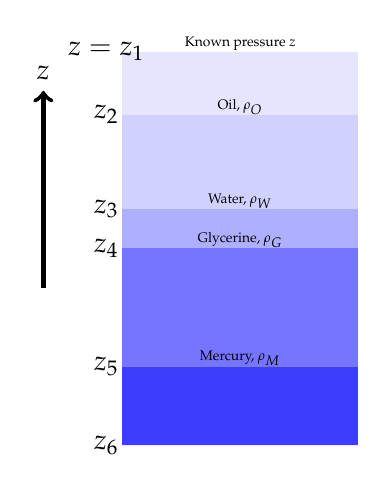
\begin{tikzpicture}
      \draw[ultra thick,->](-1,2)--(-1,4.5) node[pos=1,above]{$z$};

      \fill[white!5!blue!80](0,0)   rectangle(3,1);
      \fill[white!10!blue!60](0,1)   rectangle(3,2.5);
      \fill[white!30!blue!45](0,2.5) rectangle(3,3);
      \fill[white!40!blue!30](0,3)   rectangle(3,4.2);
      \fill[white!50!blue!20](0,4.2) rectangle(3,5);
      \node at (-.2,5) {$z=z_1$};
      \node at (-.2,4.2) {$z_2$};
      \node at (-.2,3) {$z_3$};
      \node at (-.2,2.5) {$z_4$};
      \node at (-.2,1) {$z_5$};
      \node at (-.2,0) {$z_6$};

      \node at (1.5,5.1) {\tiny Known pressure $z$};
      \node at (1.5,4.3) {\tiny Oil, $\rho_O$};
      \node at (1.5,3.1) {\tiny Water, $\rho_W$};
      \node at (1.5,2.6) {\tiny Glycerine, $\rho_G$};
      \node at (1.5,1.1) {\tiny Mercury, $\rho_M$};
    \end{tikzpicture}
    
    \column{.7\textwidth}
    For the fluid surface to remain static, the fluid pressure on both side of
    the interface have to be equal. (Obviously!) In this example:

    \vspace{-.45in}{\Large
      \begin{align*}
        p_2-p_1&=\rho_Og(z_2-z_1)\\
        p_3-p_2&=\rho_Wg(z_3-z_2)\\
        p_4-p_3&=\rho_Gg(z_4-z_3)\\
        p_5-p_4&=\rho_Mg(z_5-z_4)\\\hline
        p_5-p_1&=\sum \Delta p
      \end{align*}
    }
  \end{columns}
\end{frame}



\begin{frame}
  \frametitle{A Simple Example}
  \begin{columns}

    \column{.7\textwidth}
    \textbf{Example 1:} An aquarium is filled with water. The lateral wall of
    the aquarium is \SI{40}{cm} long and \SI{30}{cm} high. Using \SI{10}{m/s^2}
    for the acceleration due to gravity, and \SI{1}{g/cm^3} for density of
    water, the force on the lateral wall of the aquarium is:
    \begin{enumerate}[(a)]
    \item\SI{36}{N}
    \item\SI{90}{N}
    \item\SI{180}{N}
    \item\SI{1500}{N}
    \end{enumerate}

    \column{.3\textwidth}
    \pic{1}{home-fish-tank.jpg}
  \end{columns}
\end{frame}



\begin{frame}
  \frametitle{Example}
  \textbf{Example 2:} Consider the hydraulic jack in the diagram. A person
  stands on a piston that pushes down on a thin cylinder full of water. The
  cylinder is connected via pipes to a wide platform on top of which rests a
  1-ton (\SI{1000}{kg}) car. The area of the platform under the car is
  \SI{25}{m^2}; the person stands on a \SI{0.3}{m^2} piston. What is the
  lightest weight of a person who could successfully lift the car?
  \begin{center}
    \vspace{-.2in}
    \pic{.4}{jack.png}
    
    \vspace{-.2in}{\tiny Believe it or not, there \emph{is} someone who draws
      worse diagrams than Tim!}
  \end{center}
\end{frame}



\begin{frame}
  \frametitle{A ``Manometer'' Example}
  \begin{columns}

    \column{.55\textwidth}
    \textbf{Example 3:} Pressure gauge $B$ is to measure the pressure at point
    $A$ in a water flow, as shown in the figure on the right. If the pressure at
    $B$ is \SI{87}{\kilo\pascal}, estimate the pressure at $A$, in
    \si{\kilo\pascal}. Assume all fluids are at \SI{20}{\celsius}.

    \vspace{.1in}The densities of water, mercury and SAE 30 oil are,
    respectively:

    \vspace{-.3in}
    \begin{align*}
      \rho_\mathrm{water}&=\SI{1000}{kg/m^3}\\
      \rho_\mathrm{Hg}&=\SI{13600}{kg/m^3}\\
      \rho_\mathrm{oil}&=\SI{890}{kg/m^3}
    \end{align*}
    
    \column{.45\textwidth}
    \pic{1}{mano.jpg}
  \end{columns}
\end{frame}



%\begin{frame}
%  \frametitle{Hydrostatic Example: Forces on a Hinge}
%  \begin{columns}
%
%    \column{.45\textwidth}
%    \begin{tikzpicture}
%      \begin{
%    \end{tikzpicture}
%    
%    \column{.55\textwidth}
%    The gate in the figure on the left is \SI{5}{m} wide, is hinged at point
%    $B$, and rests against a smooth wall at point $A$. Compute
%    \begin{enumerate}[(a)]
%    \item the force on the gate due to seawater pressure, and
%    \item the horizontal force $P$ exerted by the wall at point $A$, and
%    \item the reaction at the hinge $B$
%    \end{enumerate}
%  \end{columns}
%\end{frame}



\begin{frame}
  \frametitle{Buoyancy}
  \framesubtitle{Everything Floats a Little}
  When an object is submerged inside a fluid (e.g.\ water, air, etc), the fluid
  exerts a pressure at the surface of the object. We can integrate the pressure
  over the entire surface area $S$ to find the total force $\mb{B}$ the fluid
  exerts on the object.
  \begin{center}
    \pic{.35}{rock_fbvectors.jpg}
  \end{center}
\end{frame}



\begin{frame}
  \frametitle{Derivation of Buoyance Force}
  Integrate the pressure $p$ over the entire surface $S$ to find the total force
  $\mb{B}$, or take some knowledge of vector calculus (divergence theorem) so
  that you don't have to:

  \eq{-.25in}{
    \mb{B}
    =-\oint_S p\hat{\mb{n}}dS
    =-\iiint \nabla p dV
  }
  
  Since pressure $p=\rho gz$ is a function in $z$ only, the gradient is easy to
  compute: $\nabla p=dp/dz=\rho g\bm{\hat{k}}$, giving us

  \eq{-.1in}{
    \mb{B}
    =\rho_\mathrm{fluid}g\bm{\hat{k}}\iiint dV
    =\rho_\mathrm{fluid}gV\bm{\hat{k}}
  }
\end{frame}



\begin{frame}
  \frametitle{Derivation of Buoyance Force}
  Although the derivation required a lot of calculus, the expression of
  buoyance force is straightforward (and \emph{this} is what you need to
  remember):
  
  \eq{-.1in}{
    \boxed{\mb{B} = \rho_\mathrm{fluid}gV\bm{\hat{k}}=
      m_\mathrm{fluid}g\bm{\hat{k}}}
  }
  
  where $\rho_\mathrm{fluid}$ is the density of the displaced fluid, and
  $V$ is the volume displaced. This equation is known as
  \textbf{Archimedes' principle}.
  
  \vspace{.25in}\textbf{Buoyance force has a magnitude that equals to the
    weight of the fluid displaced by the submerged object, pointing upward.}
\end{frame}



\begin{frame}
  \frametitle{An Easier Explanation of Buoyancy}
  \framesubtitle{Not Much Calculus}
  \begin{columns}
    \column{.7\textwidth}
    There is a simpler way to find the buoyance force, by taking an
    infinitesimal ``tube'' of the object, and finding the pressure difference
    between the top and bottom of the tube:

    \vspace{-.5in}{\Large
      \begin{align*}
        \mb{B}&=\int (p_2-p_1)dA\\
        &= \rho_\mathrm{fluid} g\int(z_2-z_1)dA\\
        &=\rho_\mathrm{fluid} g V
      \end{align*}
    }

    \vspace{-.2in}which is the same expression that we got with calculus.

    \column{.3\textwidth}
    \pic{1}{buoyancy.jpg}
  \end{columns}
\end{frame}



\begin{frame}
  \frametitle{Buoyancy}
%  Buoyancy depends on:
%  \begin{itemize}
%  \item the density of the (displaced) fluid $\rho_\mathrm{fluid}$
%  \item the volume of the fluid displaced $V$, and
%  \item the local acceleration due to gravity $g$
%  \end{itemize}
  Note that buoyancy does not depend on:
  \begin{itemize}
  \item the mass of the immersed object, or
  \item the density of the immersed object
  \end{itemize}
%\end{frame}
%
%\begin{frame}
%  \frametitle{Buoyancy}
  \vspace{.15in}Objects immersed in a fluid have an ``apparent weight''
  $\mb{W}'$ that is reduced by the buoyance force:

  \eq{-.2in}{
    \mb{W}' = \mb{W}-\mb{B}=\rho'\mb{g}V
  }
  
  where $\rho'=\rho_{\textrm{obj}}-\rho_{\textrm{fluid}}$ is the relative density
\end{frame}

%\begin{frame}
%  \frametitle{Buoyancy}
%  For a submerged object:
%  \begin{center}
%    \begin{tabular}{c|c|c|c}
%      \rowcolor{pink}
%      Densities	&
%      $B>W_{\textrm{obj}}$ &
%      $B=W_{\textrm{obj}}$ &
%      $B<W_{\textrm{obj}}$ \\\hline
%      $\rho_{\textrm{obj}}<\rho_{\textrm{fluid}}$ & object rises & float on surface & \\
%      $\rho_{\textrm{obj}}=\rho_{\textrm{fluid}}$ & & neutral buoyancy & \\
%      $\rho_{\textrm{obj}}>\rho_{\textrm{fluid}}$ & & & object sinks
%    \end{tabular}
%  \end{center}
%\end{frame}


\begin{frame}
  \frametitle{How Submarines Work}
  \framesubtitle{Like this?}
  \begin{center}
    \pic{.7}{EbHMOXk.jpg}
  \end{center}
\end{frame}



\begin{frame}
  \frametitle{How Submarines Work}
  Like all ships, a submarine does not naturally sink due to buoyancy. When a
  submarine submerges, water needed to be pumped into the  ``ballast tanks'' in
  the hull to make the ship heavier.
  \begin{center}
    \pic{1}{risinglemur.jpg}
  \end{center}
\end{frame}



\begin{frame}
  \frametitle{Stable? Or unstable?}
  Buoyance force $\mb{B}$ acts at the \emph{center of buoyancy} (CB) of a
  submerged object
  \begin{itemize}
  \item The CB is the CG \emph{if the object has constant density} and is
    fully submerged
  \item The actual CG of the object may be at a different position
  \item Sometimes the object is not fully submerged
  \end{itemize}
  
  $\mb{F}_g$ and $\mb{B}$ may act at different points, creating a torque/moment
  on the object
  \begin{center}
    %\vspace{-.15in}
    \pic{.5}{stable-unstable.jpg}
  \end{center}
\end{frame}



\begin{frame}
  \frametitle{Example}
  \begin{columns}

    \column{.7\textwidth}
    \textbf{Example 4:} An apple is held completely submerged just below the
    surface of a container of water. The apple is then moved to a deeper point
    in the water. Compared with the force needed to hold the water just below
    the surface, what is the force needed to hold it at a deeper point?
    \begin{enumerate}[(a)]
    \item Larger
    \item The same
    \item Smaller
    \item Impossible to determine
    \end{enumerate}

    \column{.3\textwidth}
    \pic{1}{apple.jpg}
  \end{columns}
\end{frame}



\begin{frame}
  \frametitle{Example}

  \begin{columns}

    \column{.4\textwidth}
    \pic{1}{hpa_b.jpg}

    \column{.6\textwidth}
    \textbf{Example 5:} A salvage ship tries to raise a sunken miniature
    submarine from the bottom of Lake Superior. The submarine and its contents
    have a mass of \SI{72000}{kg} and a volume of \SI{18.9}{m^3}. What upward
    force must be applied to raise the submarine? The density of water is
    \SI{1000}{kg/m^3}.
    \begin{enumerate}[(a)]
    \item\SI{1.8e5}{\newton}
    \item\SI{2.0e5}{\newton}
    \item\SI{4.8e5}{\newton}
    \item\SI{5.2e5}{\newton}
    \end{enumerate}
    
  \end{columns}
\end{frame}



\begin{frame}
  \frametitle{Fluid Flow}

  \begin{center}
    As important as it is to understand hydrostatics,\\
    it's way more interesting when the fluid is moving!
  \end{center}
\end{frame}


\begin{frame}
  \frametitle{Control Volume and Control Surfaces}
  A control volume ``CV'' is a fixed volume in which fluid is able to flow in
  and out of it. The surfaces of the control volume is called the control
  surface ``CS''.
  \begin{center}
    \pic{.5}{CV-CS.jpg}
  \end{center}
\end{frame}

\begin{frame}
  \frametitle{Fluid Flow: Continuity}
  In a CV, we can quantify how fluid mass changes inside:
  \begin{center}
    \textbf{rate of decrease in mass in the CV = mass flux out of the CV}
  \end{center}

  The fluid mass in the CV is the integral of density over the volume:

  \eq{-.2in}{ \int_{CV}\rho dV }
  
  The rate of decrease is therefore the negative of the time derivative:
  
  \eq{-.25in}{
    -\frac{\partial}{\partial t}\int_{CV}\rho dV
  }
\end{frame}



\begin{frame}
  \frametitle{Fluid Flow: Continuity}
  The mass flux out of the surfaces of the control volume the volume flux
  multiplied by the fluid density at the surface:

  %Applying the divergence theorem, we can convert this surface interested

  \eq{-.2in}{ \int_{CS}\rho\mb{v}\cdot d\mb{A} }
  
  Combining the LHS and RHS terms, we have the \emph{integral} form of the
  continuity equation:

  \eq{-.2in}{\boxed{
      \int_{CV}\frac{\partial\rho}{\partial t}dV +
      \int_{CS}\rho\mb{v}\cdot d\mb{A}=0
  }}
\end{frame}


\begin{frame}
  \frametitle{Fluid Flow: Continuity}
  With some clever use of vector calculus, we get the \emph{differential form}
  of the continuity equation:

  \eq{-.2in}{
    \frac{\partial\rho}{\partial t} + \nabla\cdot(\rho\mb{v})=0
  }

  \ldots which is still too difficult. So in AP Physics we usually only look at
  simple cases where
  \begin{itemize}
  \item Steady flow (time independent)
  \item Constant density
  \item Flow perpendicular to control surfaces
  \end{itemize}
\end{frame}



\begin{frame}
  \frametitle{Inlet Outlet Flow}
  \begin{center}
    \pic{.5}{physicsbook_fluids_graphik_26.png}
  \end{center}
  In this example, the mass flowing at the inlet is the same as the flow out of
  it:

  \eq{-.2in}{\boxed{\rho_1 v_1A_1=\rho_2 v_2A_2}}
  
  \vspace{-.15in}And if fluid density is constant (incompressible flow), the
  $\rho$ terms on both sides of the equation will cancel:

  \eq{-.3in}{\boxed{v_1A_1=v_2A_2}}
\end{frame}



\begin{frame}
  \frametitle{Example: Multiple Inlet \& Outlets}
  \begin{columns}

    \column{.43\textwidth}
    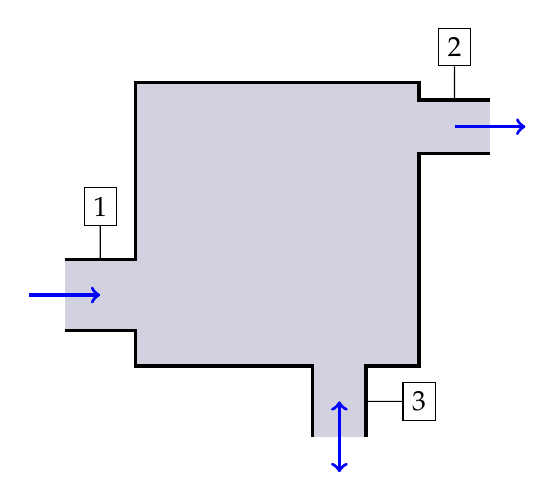
\begin{tikzpicture}[scale=.9]
      \fill[blue!20!gray!30](0,0) rectangle(4,4);
      \fill[blue!20!gray!30](2.5,0) rectangle(3.25,-1);
      \fill[blue!20!gray!30](-1,.5) rectangle(0,1.5);
      \fill[blue!20!gray!30](4,3) rectangle(5,3.75);
      \draw[very thick](-1,1.5)--(0,1.5)--(0,4)--(4,4)--(4,3.75)--(5,3.75);
      \draw[very thick](-1,0.5)--(0,0.5)--(0,0)--(2.5,0)--(2.5,-1);
      \draw[very thick](3.25,-1)--(3.25,0)--(4,0)--(4,3)--(5,3);
      \node[draw] at (-.5,2.25) (a) {1};
      \node[draw] at (4.5,4.5) (b) {2};
      \node[draw] at (4,-.5) (c) {3};
      \draw(-.5,1.5)--(a);
      \draw(4.5,3.75)--(b);
      \draw(3.25,-.5)--(c);
      \draw[->,very thick,blue](-1.5,1)--(-.5,1);
      \draw[->,very thick,blue](4.5,3.375)--(5.5,3.375);
      \draw[<->,very thick,blue](2.875,-.5)--(2.875,-1.5);
    \end{tikzpicture}

    \column{.57\textwidth}
    \textbf{Example 6:} Water at \SI{20}{\celsius} flows steadily through a
    closed tank, as shown in the figure. As section 1, $D_1=\SI{6}{cm}$ and
    the volume flow is \SI{100}{m^3/h}. At section 2, $D_2=\SI{5}{cm}$ and the
    average velocity is \SI{8}{m/s}. If $D_3=\SI{4}{cm}$, what is
    \begin{enumerate}
    \item the flow rate $Q_3$ in \si{m^3/h}?
    \item the average $v_3$ in \si{m/s}?
    \end{enumerate}
  \end{columns}
\end{frame}



\begin{frame}
  \frametitle{Governing Equations for Fluid Dynamics}

  To properly describe fluid flows, there are three conservation equations:
  \begin{itemize}
  \item continuity
  \item momentum, and
  \item energy
  \end{itemize}
\end{frame}

\begin{frame}
  \frametitle{Fluid Flow: Momentum \& Energy Equations}
  In the momentum equation, the rate of decrease of total fluid momentum inside
  the control volume CV is the net momentum flux of the fluid out of the CV
  all the forces (pressure, body, shear) acting on the fluid:

  \eq{-.15in}{
    \frac{\partial(\rho\mb{v})}{\partial t} +
    \nabla(\rho\mb{v}\otimes\mb{v}) = -\nabla p +\mb{f}+\mu\nabla^2\mb{v}
  }
  
  \vspace{-.1in}(This is even more complicated than the continuity equation, so
  thankfully you won't need this equation for AP Physics!)

  \vspace{.2in}The energy equation follows a similar thought process as the
  previous two equations, but the terms are even more complicated.

\end{frame}



\begin{frame}
  \frametitle{Navier-Stokes Equations}
  Together, the three conservation equations are called the
  \textbf{Navier-Stokes equations}. In differential form, they are usually
  written as:
  
  \vspace{-.4in}{\Large
    \begin{align*}
      \frac{\partial\rho}{\partial t} + \nabla\cdotp(\rho\mb{v})&=0\\
      \frac{\partial(\rho\mb{v})}{\partial t} +
      \nabla(\rho\mb{v}\otimes\mb{v}) &= -\nabla p +\mb{f}+\mu\nabla^2\mb{v}\\
      \frac{\partial e}{\partial t} + \nabla\cdotp(e\mb{v})&=
      -\nabla\cdotp p +\frac{1}{Re\; Pr}\nabla q +
      \frac{1}{Re}\nabla\cdotp(\tau\cdotp\mb{v})
    \end{align*}

  }

  Even for a 2nd-year engineering student experienced with calculus, solving
  the N-S equations is still a daunting task, so let's make some assumptions!
\end{frame}



\begin{frame}
  \frametitle{Let's Make Some Assumptions}
  \framesubtitle{For an ``ideal fluid flow''}
  The flow is \textbf{steady}
  \begin{itemize}
  \item Flow is ``time independent'', i.e.\ does not change with time
  \item All derivatives w.r.t.\ time are zero
  \end{itemize}

  The flow is \textbf{inviscid}
  \begin{itemize}
  \item The fluid has no viscosity
  \item No friction between the fluid and the surrounding, and therefore
  \item No shear stresses on the fluid
  \item Only forces are pressure at the surface, and body forces from gravity
  \end{itemize}

  The flow is \textbf{incompressible}
  \begin{itemize}
  \item Density is constant throughout
  \item The compressibility of fluid usually depends on its flow velocity,
    at Mach number of $M\approx 0.3$, fluid becomes incompressible
  \end{itemize}
\end{frame}



\begin{frame}
  \frametitle{Let's Make Some Assumptions}
  \framesubtitle{For an ``ideal fluid flow''}
  We will also assume that
  \begin{itemize}
  \item there is \textbf{no shaft work} done along the streamline
  \item there is \textbf{no heat transfer} along the streamline
  \end{itemize}
  Then the N-S equations reduces to the
  \textbf{Bernoulli equation}
  
  \eq{-.1in}{\boxed{
      p_1+\frac{1}{2}\rho v_1^2 + \rho gz_1=
      p_2+\frac{1}{2}\rho v_2^2 + \rho gz_2
    }
  }
  
  The term $\displaystyle\frac{1}{2}\rho v^2$ is called ``dynamic pressure'',
  and $\rho gz$ is the ``hydrostatic pressure''
\end{frame}



%\begin{fame}
%  \frametitle{Flow Continuity}
%  Usually the continuity equation is written in \emph{differential form}, by
%  applying the \emph{divergence theorem} to the flux term:
%
%  \vspace{-.3in}{
%    \begin{align*}
%      \int_{CV}\frac{\partial\rho}{\partial t}dV+
%      \int_{CS}\rho\mb{v}\cdot d\mb{A}=&0\\
%    \end{align*}
%  }
%\end{frame}
%  \eq{-.15in}{
%    \boxed{\Phi_\mathrm{V}=\int\mb{V}\cdot d\mb{A}}
%  }
%    
%  \vspace{-.1in}where $\mb{V}$ is the velocity (vector field) at the surface,
%  and $d\mb{A}$ is the infinitesimal area pointing \textbf{outwards}. We can
%  also expressed volume flux using the outward normal unit vector
%  $\hat{\mb{n}}$:
%
%  \eq{-.15in}{
%    \boxed{\Phi_\mathrm{V}=\int\mb{V}\cdot\hat{\mb{n}}dA}
%  }
%\end{frame}
%
%\begin{frame}
%  \frametitle{Bernoulli Equation}
%
%  \eq{-.01in}{\boxed{
%      p_1+\frac{1}{2}\rho v_1^2 + \rho gz_1=
%      p_2+\frac{1}{2}\rho v_2^2 + \rho gz_2
%  }}
%\end{frame}
%
%
%\begin{frame}
%  \frametitle{Bernoulli Equation}
%
%  \eq{-.01in}{\boxed{
%      p_1+\frac{1}{2}\rho v_1^2 + \rho gz_1=
%      p_2+\frac{1}{2}\rho v_2^2 + \rho gz_2
%  }}
%
%  Bernoulli's equation is valid when
%  \begin{itemize}
%  \item the flow is \textbf{steady} (independent of time)
%  \item the flow is \textbf{incompressible}--compressibility (i.e. changes in
%    density of the fluid) effects are negligible for Mach number $M<0.30$
%  \item the flow \textbf{along a single streamline}
%  \item there is \textbf{no shaft work} done along the streamline between 1 and
%    2
%  \item there is \textbf{no heat transfer} along the streamline between 1 and 2
%  \end{itemize}
%\end{frame}



\begin{frame}
  \frametitle{Bernoulli Equation}

  Regions where Bernoulli equation is valid:
  \begin{center}
    \pic{.8}{bernoulli.jpg}
  \end{center}
\end{frame}



\begin{frame}
  \frametitle{Example}

  \textbf{Example 7:} Find a relation between the nozzle discharge velocity
  $V$ and the tank free-surface height $h$. Assume frictionless flow.
  \begin{center}
    \pic{.4}{EGL.jpg}
  \end{center}

  \vspace{-.2in}{
    \footnotesize (The line labelled ``EGL'' is called the
    ``energy grade line'', or the ``Bernoulli head'', given by the equation
    $h_0=z+p/\rho g+v^2/2g$. In the region where Bernoulli equation is valid,
    EGL is a constant.)\par
  }
\end{frame}
%
%
%
%\begin{frame}
%  \frametitle{How Does A Wing Work?}
%
%  When air flows past a wing, a force is generated
%\end{frame}
%
%\end{document}
